\section{Synthetic measurement from circular-channel counts}
\label{sec:count-measurement}
The original detector study uses the computed complex fields at $R_0=24,96$,
$\eta=0.35,0.7$, and $m=1,2,4$; the focused diagnosis below adds $m=3$
without replacing the original records. The true circular-channel intensities,
$I_\pm=|U_{m\mp1}|^2/2$, are normalized by the incident transverse power.
These are synthetic conditions; no camera, translation stage, or experimental
performance is inferred from them. Unit detection efficiency is assumed in
the reference count $N$ per axial plane. A different known efficiency can be
absorbed into $N$.

Before counting, each intensity is convolved with a circular Gaussian
point-spread function. For a radial intensity the convolution is evaluated as
\begin{equation}
 I_\sigma(r)=\int_0^\infty I(s)\frac{s}{\sigma^2}
 e^{-(r-s)^2/(2\sigma^2)} I_{0e}(rs/\sigma^2)\,\mathrm{d}s,
\end{equation}
where $I_{0e}(t)=e^{-t}I_0(t)$ is the scaled modified Bessel function.
Each square detector pixel is then integrated using $3\times3$
Gauss--Legendre quadrature. The circular aperture contains pixels whose
centres lie within the nominal proxy radius. It therefore includes finite
pixel sampling of the aperture as well as averaging within each pixel.
Tests with $5\times5$ and $7\times7$ quadrature changed the pilot half-height
positions by less than $2\times10^{-8}$ in $\tau$. The radial convolution
agreed with an independently known Gaussian-convolution solution to
$2.93\times10^{-9}$ in relative $L^2$ error.

Let $p_{\pm j}$ be the resulting fraction of incident power in pixel $j$.
The count means, before background subtraction, are
\begin{align}
 \lambda_{+j}&=N(1+g)[(1-a)p_{+j}+b p_{-j}]+B,\\
 \lambda_{-j}&=N(1-g)[a p_{+j}+(1-b)p_{-j}]+B,
 \qquad a=c+\delta/2,\quad b=c-\delta/2.
\end{align}
Independent Poisson counts and additive Gaussian read noise are generated
for the two channels. The baseline has $N=10^6$ reference counts per plane,
axial step $0.1$ mm, pixel pitch $1\,\mu$m, blur standard deviation
$1\,\mu$m, read-noise standard deviation one electron per pixel, and
background $B=0.1$ electron per pixel. The gain standard deviation is
$0.1\%$ with cross-order correlation $0.8$. The two background calibration
offsets have standard deviation $0.001$ electron per pixel and correlation
$0.5$, and are shared across scans. The mean polarimetric mixing is
$c=0.002$, with shared asymmetry standard deviation $0.0002$.
The monitor has mean $100N$ and independent Poisson noise at each plane,
shared across the compared orders.

The common axial offset has standard deviation $0.02$ mm. Independent
order-specific offsets have standard deviation $0.01$ mm, and independent
linear scan drifts have standard deviation $0.01$ mm at the scan endpoints.
For every realization, the intensity is evaluated at the displaced physical
plane while the aperture remains at its nominal position. Shifting only
the already integrated moving-aperture curve would describe a different
measurement and is not used.

Since the aperture weights are binary, the sum of independent Poisson pixel
counts is exactly Poisson with mean $\sum_j\lambda_{\pm j}$. We use this
identity to simulate the aggregate channel counts, with read variance equal
to the number of retained pixels times the per-pixel variance. This retains
the count statistics of the full image without drawing every pixel in every
realization. Representative full raw channel images and aggregate count
traces are retained in the data archive. Noise is never added as a prescribed
percentage of the final $Q$.

The scan covers $-1.5\leq\tau\leq2.5$. A cubic Savitzky--Golay filter uses
a nominal width $0.25$ in $\tau$, rounded to an odd number of samples with
at least five points. The estimator selects the largest interior smoothed
maximum within $0.2\leq\tau\leq1.8$, records all additional maxima, and
uses a three-point quadratic peak value. The half-height event is the
nearest preceding rising linear crossing. Negative counts are retained.
A missing maximum or crossing is an extraction failure; returning a number
does not imply that the correct physical peak was selected.

The linearized confidence interval propagates the full covariance through
the smoothing matrix and the peak/crossing functional. It retains
peak--crossing covariance, shared monitor and calibration errors, and
cross-order axial errors. For this simulation benchmark the covariance is
evaluated at the known expected detector signal. It is therefore an
\emph{expected-signal linearization}, not a claim that these parameters can be
estimated without calibration in an experiment. Bias and coverage are
reported separately against the ideal continuous-aperture event and the
noise-free pixel-and-blur event. Unknown systematic gain bias is not absorbed
into a random-error interval.

The design contains 96 scenarios with 1000 realizations each: marginal
sweeps of $N=10^4$--$10^7$, axial steps $0.05$--$1$ mm, gain standard
deviation $0$--$1\%$, blur $0$--$5\,\mu$m, pixel pitch
$0.5$--$4\,\mu$m, read noise $0$--$3$ electrons, and independent axial
offset $0$--$0.1$ mm, together with two predefined interacting/systematic
stress scenarios. These ranges define marginal sweeps rather than a full
Cartesian product. The scenario table reports event statuses as source data.
Four representative conditions were repeated independently with 4000
realizations. For $R_0=96$, $\eta=0.7$, $m=4$, the correct-sign fractions
were $0.251$ and $0.255$ at $N=10^6$, and $0.979$ and $0.98075$ at
$N=10^7$. These repetitions support the distinction between those two
count regimes; they do not establish a universal detection threshold.

\begin{table}[htbp]
\centering\small
\caption{Baseline synthetic measurement for $m=4$ relative to $m=1$.
Bias and interval coverage refer to the ideal continuous-aperture advance.
Widths are the full linearized 95\% interval; the correct-sign fraction is empirical.}
\label{tab:measurement-baseline}
\begin{tabular}{rrrrrrr}\toprule
$R_0$ & $\eta$ & $\Delta z_4$ (mm) & Bias (mm) & Width (mm) & Coverage & Correct sign\\\midrule
24 & 0.35 & 3.69334 & $-0.00314$ & 0.2363 & 0.957 & 1.000 \\
24 & 0.7 & 3.78726 & $-0.02302$ & 0.5604 & 0.950 & 1.000 \\
96 & 0.35 & 0.45746 & $-0.01091$ & 0.6265 & 0.955 & 0.994 \\
96 & 0.7 & 0.48972 & $-1.71029$ & 8.3827 & 0.915 & 0.251 \\
\bottomrule\end{tabular}
\end{table}

\begin{figure}[p]
\centering
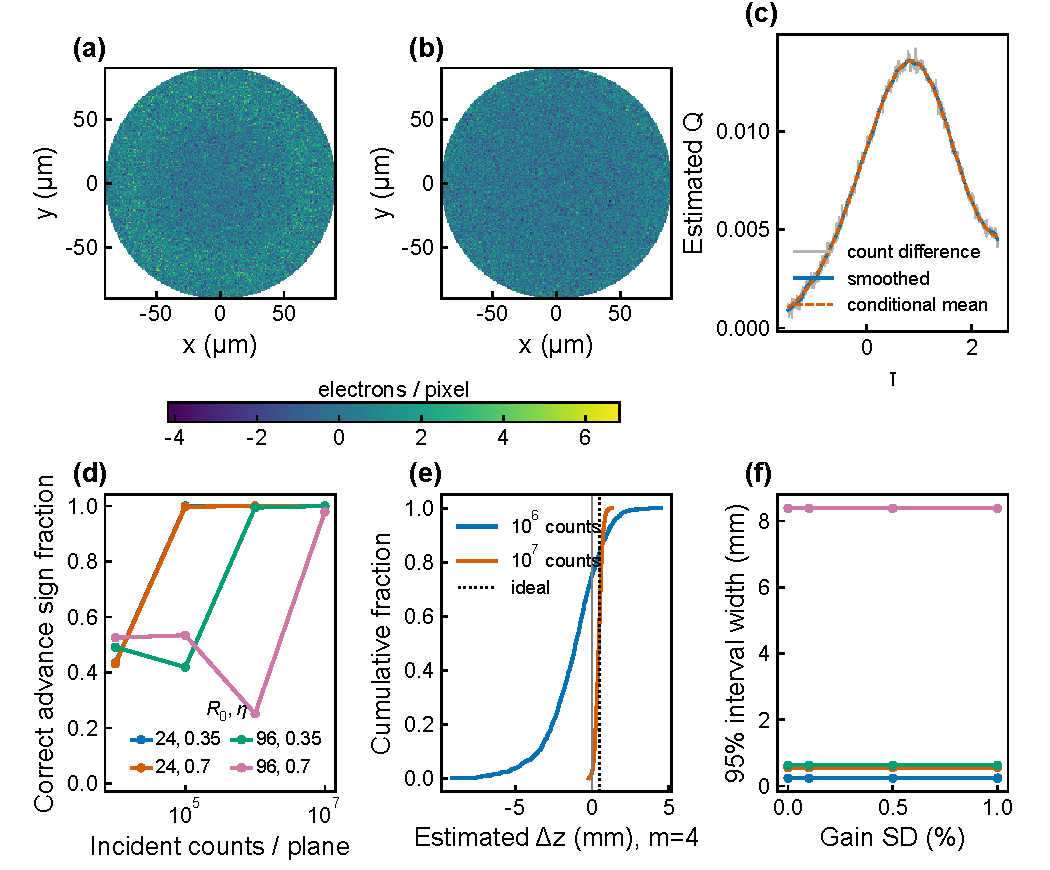
\includegraphics[width=\linewidth]{../figures/synthetic_measurement.pdf}
\caption{Synthetic count-level measurement. (a,b) Independently generated
raw circular-channel images at $\tau=0$, $R_0=24$, $\eta=0.7$, $m=4$,
with the same electron-count scale. (c) One aggregate count trace,
its smoothed estimate, and the conditional mean. (d) Correct-sign fraction
for $\Delta z_4$ in the count sweep with other conditions fixed.
(e) Full empirical cumulative distributions at $R_0=96$, $\eta=0.7$;
the dotted line is the ideal continuous-aperture advance.
(f) Linearized interval widths with the stated gain covariance.
All quantities are simulated, and each sweep point contains 1000 realizations.}
\label{fig:synthetic-measurement}
\end{figure}

For the baseline at $R_0=24$, both tested non-reference orders have the
correct advance sign in all 1000 realizations. At $R_0=96$, $\eta=0.7$,
however, the ideal $m=4$ advance is $0.48972$ mm and the estimated mean
is biased by $-1.71029$ mm. Only $25.1\%$ of realizations have the correct
sign. The failure is associated with low local counts and peak selection
under noise, rather than the absence of a mathematical crossing in the
ideal signal. In the combined low-count/coarse-image stress case,
$2.5\%$ of paired estimates cannot be extracted, while the sign fraction
among extracted estimates is approximately $0.502$. Very wide linearized
intervals in this regime are not evidence of a useful measurement.

\subsection{Four-stage failure diagnosis and frozen estimator comparison}
Before drawing the focused random samples, we fixed three extraction rules:
(i) the retained width-$0.25\tau$ blind largest-peak estimator; (ii) a
known-peak-location-assisted diagnostic using the same smoothing but selecting
the local maximum nearest the known noiseless detector peak; and (iii) one implementable blind
alternative using a pre-fixed width $0.75\tau$ and the largest peak. The
third rule uses neither the true displacement nor $D_m$. One thousand
calibration replicates determine the covariance, and 3000 independent
validation replicates determine bias, extraction, interval coverage, and
sign recovery. The protocol and seeds are stored before the validation draws.

Four stages isolate the failure. A is the continuous-field event in the
specified ROI. B applies pixel integration and blur without random noise.
C applies the fixed smoothing and peak/crossing routine to the noiseless
detector curve. D applies the same routine to the raw random channel counts.
For the difficult $R_0=96$, $\eta=0.7$, $m=4$ case, A--D give
$0.489722$, $0.484247$, $0.484237$, and $-1.242756$ mm for the retained
blind method at $N=10^6$. The imaging bias is $-0.005475$ mm and the
deterministic estimator bias is $-0.000010$ mm, whereas the random bias from
C to D is $-1.726993$ mm. The original 1000- and 4000-realization results
are therefore corroborated without being overwritten.

The estimator returns a number in every focused validation scan, so all-run
and extracted-only fractions coincide here. At $N=10^6$, the retained blind
and location-assisted rules select the same discrete local maximum in only
$14.9\%$, $13.6\%$, and $13.0\%$ of the $m=2,3,4$ scans. Equality of these
sample indices does not establish that either selected the same physical peak
branch. The retained rule gives correct-sign fractions of $42.0\%$, $32.0\%$,
and $25.7\%$; the location-assisted diagnostic gives only $47.4\%$, $42.7\%$,
and $38.4\%$. This diagnostic uses the noiseless peak location but leaves the
noisy peak value, physical branch, and rising crossing free, so its residual
error cannot be attributed uniquely to the crossing. The wider blind rule
improves the fractions to $50.9\%$, $52.5\%$, and $54.9\%$, still insufficient
for a feasibility claim.

At the detector half-height and $N=10^6$, the expected $(I_+,I_-)$ ROI
counts are $(85.81,6.83)$ for $m=1$ and $(163.44,29.75)$ for $m=4$.
The aperture contains hundreds to thousands of pixels depending on order,
so one electron of independent read noise per pixel accumulates in the
aggregate. A Poisson-only ablation gives retained-estimator sign fractions
$68.9\%$, $85.1\%$, and $94.0\%$ for $m=2,3,4$. Counting plus read noise
reduces them to $43.5\%$, $37.1\%$, and $26.9\%$, reproducing most of the
full failure; counting plus background alone gives $57.5\%$, $65.2\%$,
and $67.3\%$. Hence the dominant modeled cause is accumulated read noise,
with peak/crossing selection converting it into order-dependent bias;
background adds degradation. It is not accurately described as incident
photon shortage alone.

At $N=10^7$, the retained estimator gives correct signs in $74.6\%$,
$91.9\%$, and $97.6\%$ of the $m=2,3,4$ scans, and the pre-fixed wider
rule gives $86.5\%$, $99.1\%$, and $99.9\%$. The smaller $m=2$ shift
remains more difficult. At $R_0=24$ and $N=10^6$, all $m=2,3,4$ signs
are recovered for both tested apodizations under the retained estimator.
These outcomes are conditional on the stated synthetic detector and do not
set a general photon or hardware threshold.

\begin{table}[htbp]
\centering\scriptsize
\caption{Four-stage diagnosis at $R_0=96$, $\eta=0.7$, and $N=10^6$ for the retained blind estimator. A is the continuous-field event, B includes noiseless pixel and blur response, C applies the fixed smoothing and peak rule to B, and D is the mean over 3000 independent count-level validation scans. Values are millimeters except the final percentage.}
\label{tab:measurement-stages}
\begin{tabular}{r@{\quad}rrrrrrrr}
\toprule
$m$ & A & B & C & D & B$-$A & C$-$B & D$-$C & sign (\%) \\
\midrule
2 & 0.149997 & 0.137186 & 0.137255 & $-0.304859$ & $-0.012811$ & $+0.000069$ & $-0.442114$ & 42.0 \\
3 & 0.314388 & 0.311861 & 0.311892 & $-0.715232$ & $-0.002527$ & $+0.000030$ & $-1.027124$ & 32.0 \\
4 & 0.489722 & 0.484247 & 0.484237 & $-1.242756$ & $-0.005475$ & $-0.000010$ & $-1.726993$ & 25.7 \\
\bottomrule
\end{tabular}
\end{table}

\begin{table}[htbp]
\centering\scriptsize
\caption{Estimator comparison for the difficult $R_0=96$, $\eta=0.7$ condition. Sign percentages and random-mean advances use 3000 independent validation scans. The location-assisted diagnostic selects the noisy local maximum nearest the known noiseless peak location; it does not fix the noisy peak value, physical branch, or half-height crossing. The wide estimator is a pre-frozen blind rule.}
\label{tab:measurement-estimators}
\begin{tabular}{rcrrr@{\qquad}rrr}
\toprule
& & \multicolumn{3}{c}{correct sign (\%)} & \multicolumn{3}{c}{mean advance (mm)}\\
$N$ & estimator & $m=2$ & $m=3$ & $m=4$ & $m=2$ & $m=3$ & $m=4$ \\
\midrule
$10^{6}$ & current & 42.0 & 32.0 & 25.7 & $-0.305$ & $-0.715$ & $-1.243$ \\
$10^{6}$ & location assisted & 47.4 & 42.7 & 38.4 & $-0.119$ & $-0.315$ & $-0.590$ \\
$10^{6}$ & wide & 50.9 & 52.5 & 54.9 & 0.048 & 0.071 & 0.135 \\
$10^{7}$ & current & 74.6 & 91.9 & 97.6 & 0.126 & 0.289 & 0.449 \\
$10^{7}$ & location assisted & 73.3 & 91.4 & 97.7 & 0.130 & 0.302 & 0.473 \\
$10^{7}$ & wide & 86.5 & 99.1 & 99.9 & 0.132 & 0.303 & 0.473 \\
\bottomrule
\end{tabular}
\end{table}


\begin{figure}[p]
\centering
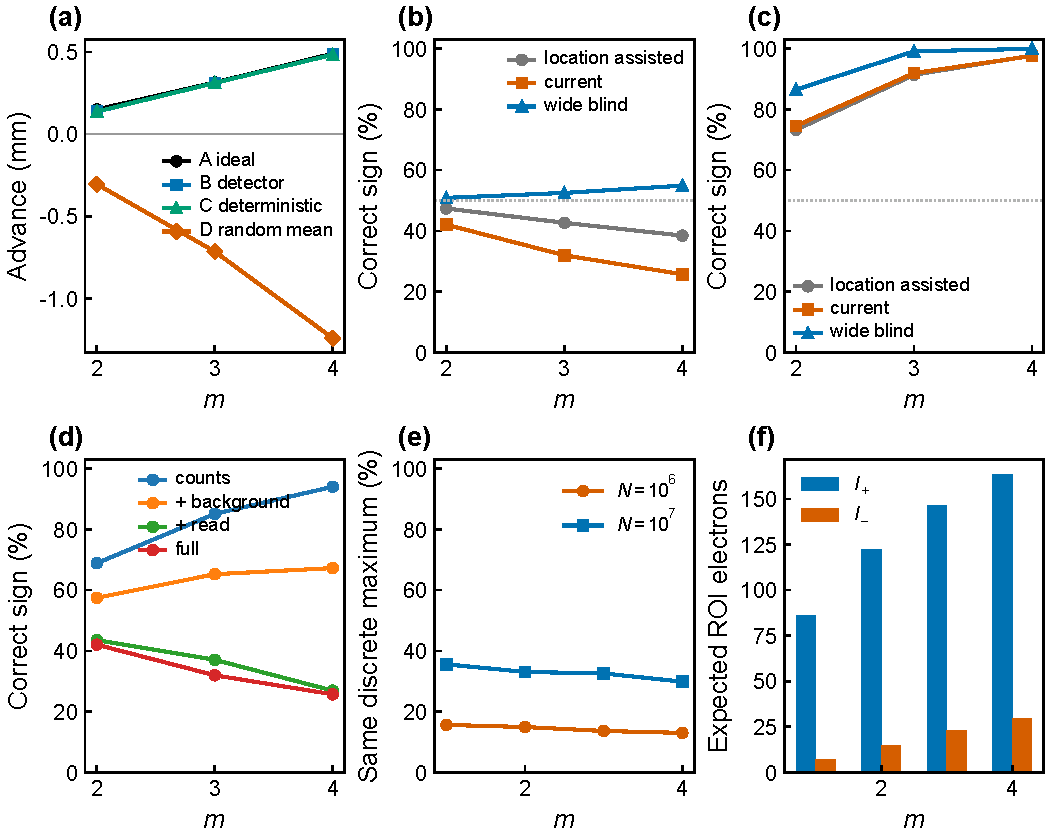
\includegraphics[width=\linewidth]{../figures/focused_measurement_diagnosis.pdf}
\caption{Focused diagnosis of the difficult $R_0=96$, $\eta=0.7$
measurement. (a) Continuous-field (A), noiseless detector (B), deterministic
estimator (C), and random validation mean (D) for the retained blind rule.
(b,c) Correct-sign fractions for the location-assisted diagnostic, retained blind, and pre-fixed wider
blind estimators at $10^6$ and $10^7$ reference counts per plane.
(d) Noise-source ablations at $10^6$ counts for the retained estimator.
(e) Fraction for which the retained blind and location-assisted rules select
the same discrete local maximum; this is not a physical peak-identity label.
(f) Expected circular-channel ROI counts at
the noiseless detector half-height for $10^6$ incident reference counts.
Each focused fraction uses 3000 independent validation scans; the assisted
rule is diagnostic and the wider blind rule was fixed before those scans.}
\label{fig:focused-measurement}
\end{figure}
\FloatBarrier

\subsection{Proposed channel-resolved optical implementation}

Figure~\ref{fig:proposed-experiment} maps the modeled observable to a
laboratory measurement. A linearly polarized continuous-wave source at
$632.8$~nm is spatially filtered and expanded before a polarization
Mach--Zehnder interferometer. The two arms use phase-only spatial-light-
modulator holograms with Fourier filtering to encode the same finite-energy
circular Airy envelope $f_{\mathrm A}(r)$ and the charges $q_+=m-1$ and
$q_-=m+1$. A half-wave plate and the hologram efficiencies set the incident
channel powers. The arms are recombined in orthogonal linear polarizations;
a quarter-wave plate at $45^\circ$ converts them to the circular basis used in
the main text. A uniform inter-arm phase changes the polarization
orientation but not $I_\pm$ or $S_3$. Transverse registration, equal radial
scale, and power balance must nevertheless be calibrated because they change
the measured channel intensities.

The acquisition head is translated through the autofocusing region, or an
equivalent translated relay images each plane. A quarter-wave plate followed
by a polarizing beam splitter sends the two circular components to synchronized
detectors. A monitor photodiode records the incident normalization. Full frames
are retained, so the scaled proxy boundary is applied digitally with physical
radius
\begin{equation}
 \rho_s(z)=\frac{2kw^3x_s}{z},\qquad x_s=j'_{m,1},
\end{equation}
rather than with a moving mechanical iris. After dark, flat-field, gain,
polarimetric-leakage, and image-registration corrections, let
$\widetilde C_{\pm j}(z)$ denote the corrected count in pixel $j$. The directly
measured traces are
\begin{align}
 \widehat Q(z)&=\frac{1}{\widehat P_{\rm in}(z)}
  \sum_{j\in{\rm ROI}(z)}[\widetilde C_{+j}(z)-\widetilde C_{-j}(z)],\\
 \widehat T(z)&=\frac{1}{\widehat P_{\rm in}(z)}
  \sum_{j\in{\rm ROI}(z)}[\widetilde C_{+j}(z)+\widetilde C_{-j}(z)],
 \qquad
 \widehat{\bar p}_3(z)=\frac{\widehat Q(z)}{\widehat T(z)}.
\end{align}
The same fixed peak and rising-crossing rules used in the count simulation
then give $z_{50}(m)$ and $\Delta z_m=z_{50}(1)-z_{50}(m)$. For the alternative
actual-zero analysis, the first positive-to-negative zero is extracted from
the calibrated, azimuthally averaged $S_3$ map at each plane and its branch
status is retained. The axial scan increment is only the sampling interval;
repeat scans and the calibrated covariance are required to determine event
uncertainty.

Input certification is kept separate from this primary acquisition. A
quarter-wave plate and rotating linear polarizer provide full-Stokes images,
whereas interference of each circularly selected component with a matched
spherical reference checks $q_+$ and $q_-$. A linear-analyzer petal pattern is
not used to infer $m$, because the fixed $P=1$ family has the same twofold
modulation for every $m$. These modules follow established SLM preparation,
Stokes-polarimetry, and circular-channel interferometry procedures
\cite{Liu2021,Yan2025,Zhu2025}. Figure~\ref{fig:proposed-experiment} is an
implementable proposal; the present work has not built this apparatus, and the
feasibility numbers above remain predictions of the stated detector model.

\begin{figure}[p]
\centering
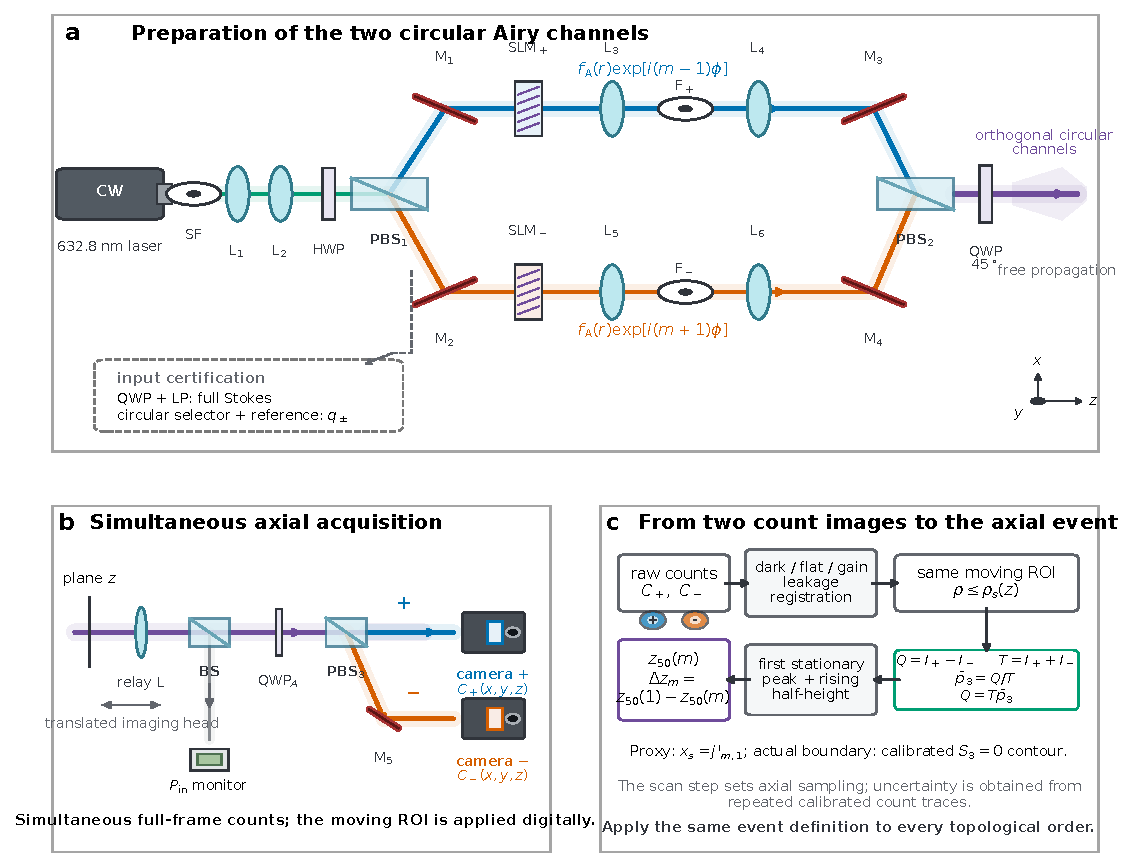
\includegraphics[width=\linewidth]{../figures/proposed_experimental_layout.pdf}
\caption{Proposed measurement of the topological-order-dependent axial event.
(a) A polarization Mach--Zehnder interferometer prepares the same circular
Airy envelope in the $q_+=m-1$ and $q_-=m+1$ arms and converts the recombined
field to orthogonal circular polarizations. The dashed branch contains
independent input diagnostics. SF, spatial filter; L1--L2, beam expander; HWP,
half-wave plate; PBS, polarizing beam splitter; SLM, spatial light modulator;
QWP, quarter-wave plate. (b) A translated imaging head separates and records
the two circular-channel count images simultaneously while a photodiode
monitors incident power. (c) Calibrated full-frame counts are integrated in
the digital moving ROI to obtain $Q$, $T$, and $\bar p_3$ before the fixed
peak and rising-half-height estimator is applied. This is a proposed optical
implementation, not an experiment performed in the present work.}
\label{fig:proposed-experiment}
\end{figure}
